\documentclass[11pt]{article}
\usepackage{fullpage}
\usepackage[utf8]{inputenc}
\usepackage{amsmath}
\usepackage{amsthm}
\usepackage{amsfonts}
\usepackage{amssymb}
\usepackage{graphicx}
\usepackage{hyperref}
\usepackage{algorithm}
\usepackage{algpseudocode}
\usepackage{listings}
\usepackage{color}
\usepackage{float}
\usepackage{tikz}
\usepackage{tikz-qtree}
\usepackage{mdframed}
\usepackage{pgfplots}
\makeatletter
\newenvironment{breakablealgorithm}
  {% \begin{breakablealgorithm}
   \begin{center}
     \refstepcounter{algorithm}% New algorithm
     \hrule height.8pt depth0pt \kern2pt% \@fs@pre for \@fs@ruled
     \renewcommand{\caption}[2][\relax]{% Make a new \caption
       {\raggedright\textbf{\ALG@name~\thealgorithm} ##2\par}%
       \ifx\relax##1\relax % #1 is \relax
         \addcontentsline{loa}{algorithm}{\protect\numberline{\thealgorithm}##2}%
       \else % #1 is not \relax
         \addcontentsline{loa}{algorithm}{\protect\numberline{\thealgorithm}##1}%
       \fi
       \kern2pt\hrule\kern2pt
     }
  }{% \end{breakablealgorithm}
     \kern2pt\hrule\relax%
   \end{center}
  }
\makeatother
\newtheoremstyle{definitionstyle}
  {3pt} % Space above
  {3pt} % Space below
  {\normalfont} % Body font
  {} % Indent amount
  {\bfseries} % Theorem head font
  {} % Punctuation after theorem head
  { } % Space after theorem head
  {} % Theorem head spec (can be left empty, meaning `normal`)

\theoremstyle{definitionstyle}
\newtheorem{defn}{Definition}
\newtheorem{thm}{Theorem}
\newtheorem{lem}{Lemma}
% \newtheorem{proof}{Proof}
\usepackage{framed}
\newenvironment{framedminipage}
    {\begin{framed}\begin{minipage}{0.9\textwidth}}
    {\end{minipage}\end{framed}}
\begin{document}
\title{A Dive to MCTS}
\author{liuhanzuo}
\date{\today}
\maketitle
\begin{abstract}
This survey explores the Monte Carlo Tree Search (MCTS) algorithm, a versatile decision-making framework with applications across various domains. It begins by reviewing the foundational concepts of Markov Decision Processes (MDP) and Monte Carlo methods, which form the basis of MCTS. The core MCTS algorithm is examined, highlighting its four main steps: selection, expansion, simulation, and backpropagation. Several MCTS variants are discussed, including reward-based, visited-based, and hybrid approaches, each balancing exploration and exploitation in unique ways. The survey also covers advanced algorithms such as Upper Confidence Bounds for Trees (UCT) and its variations, including UCB1-tuned and Bayesian UCT, emphasizing both theoretical underpinnings and practical implementations. Additionally, the integration of learning techniques like Temporal Difference (TD) learning, its Monte Carlo variant (TDMC), and Single Player MCTS (SP-MCTS) within MCTS is explored. Experimental results are presented in two parts: the first, demonstrating the effectiveness of advanced MCTS algorithms in the context of Tic-Tac-Toe; the second, introducing and comparing a new state-of-the-art experimental UCT-tuned algorithm for the Gobang game. This survey offers a comprehensive overview of MCTS and its applications, providing valuable insights for both researchers and practitioners in the field.
\end{abstract}
\section{BackGround}
\subsection{MDP}
We start the background part by introducing Markov Decision Process(MDP). The basic elements of MDP are as follows:
\begin{itemize}
    \item State Space $\mathcal{S}$: The set of all possible states.
    \item Action Space $\mathcal{A}$: The set of all possible actions.
    \item Transition Probability $T(s',s,a)$: The probability of transitioning to state $s'$ given that the current state is $s$ and the action taken is $a$.
    \item Reward Function $R(s,a,s')$: The reward received after transitioning from state $s$ to state $s'$ by taking action $a$.
\end{itemize}
The goal of MDP is to find a policy $\pi$ that maximizes the expected cumulative reward. The policy $\pi$ is a mapping from states to actions. Which indicates our strategy or policy for a given state. Here, we need to note that we usually choose the $\pi$ to mamximize the reward.
\subsection{Monte Carlo Methods}
From the MDP we can see that: when we are making a decision, what we really care about the the "expected reward" or "potential reward" for taking an action $a$ in state $s$. The Monte Carlo Methods is a class of algorithms that estimate the expected reward by sampling the environment. The basic idea is to simulate the environment and collect the reward. The expected reward is then estimated by the average of the collected rewards. The Monte Carlo Methods are widely used in reinforcement learning, game theory, and other fields.\\
To be more secific, we define the Q-value function as:
\[
    Q(s,a)=\frac{1}{N(s,a)}\sum_{i=1}^{N(s)}\mathbb{I}_{s,a}R_i
\] 
Where the definition is:
\begin{itemize}
    \item $N(s,a)$ is the number of times action $a$ has been taken in state $s$.
    \item $N(s)$ is the number of times state $s$ has been visited. i.e. $N(s)=\sum_a N(s,a)$
    \item $\mathbb{I}_{s,a}$ is the indicator function that is 1 if the action $a$ is taken in state $s$ and 0 otherwise.
    \item $R_i$ is the reward received after taking action $a$ in state $s$.
    \item $Q(s,a)$ is the estimated Q-value of taking action $a$ in state $s$ (expected reward).
\end{itemize}
At this point, we have delved into the core aspect of the system: exploration. This involves devising a strategy to effectively explore the state space and accurately estimate the Q-values, thereby determining the optimal policy. Monte Carlo Methods provide a robust approach to address this challenge.
\subsection{Advanced Works}
AlphaGo\cite{silver2017mastering}, developed by DeepMind, marks a significant advancement in artificial intelligence, particularly in game playing. It integrates Monte Carlo Tree Search (MCTS) with deep neural networks to achieve superhuman performance in Go. The neural networks evaluate board positions and suggest moves, while MCTS explores promising move sequences, effectively balancing exploration and exploitation. AlphaGo's prowess was demonstrated in its 2016 victory against top Go player Lee Sedol. Subsequently, DeepMind introduced AlphaGo Zero, which learns to play Go from scratch without human data, relying solely on self-play to train its neural networks. This approach enables the discovery of novel strategies and tactics. AlphaGo Zero's success underscores the potential of combining reinforcement learning with advanced search algorithms, heralding future AI advancements.
AlphaGo Zero, an evolution of AlphaGo, further refines the integration of MCTS with deep learning. Unlike its predecessor, which relied on human game data for training, AlphaGo Zero learns solely through self-play. It uses a deep neural network to evaluate board positions and predict move probabilities, which are then used to guide the MCTS simulations. The neural network is trained using the outcomes of these simulations, creating a feedback loop that continually improves both the network and the MCTS policy. This approach allows AlphaGo Zero to discover novel strategies and achieve superhuman performance without any human input, demonstrating the power of combining MCTS with deep reinforcement learning.
\section{Monte Carlo Tree Search}
\subsection{Introduction}
This section delves into the Monte Carlo Tree Search (MCTS) family of algorithms. MCTS is based on two core principles: approximating the true value of an action through random simulations and efficiently using these values to steer the policy towards a best-first strategy. The algorithm incrementally constructs a partial game tree, leveraging the outcomes of prior explorations to refine move value estimates. These estimates, especially for the most promising moves, become increasingly accurate as the tree expands.\\
In this section, we will detail several representative algorithms, present their results, and elucidate the underlying intuitions.
\subsection{General MCTS}
The general MCTS algorithm is as follows:
\begin{breakablealgorithm}
    \caption{General MCTS}
    \begin{algorithmic}[1]
        \Function{MCTS}{$s_0$}
            \State create a node $v_0$ with state $s_0$
            \While{within computational budget}
                \State $v_l\gets$\Call{TreePolicy}{$v_0$}, $\Delta\gets$\Call{DefaultPolicy}{$s(v_l)$}
                \State \Call{Backup}{$v_l,\Delta$}
            \EndWhile
            \State \Return \Call{BestChild}{$v_0$}
        \EndFunction
    \end{algorithmic}
    \label{alg:general_mcts}
\end{breakablealgorithm}
Basically, we have four steps:
\begin{enumerate}
    \item \texttt{Selection}: Start from the root point, we use a policy -- child selecting policy to select the next node to expand. (run the \texttt{TreePolicy} function)
    \item \texttt{Expansion}: Expand the selected node and get the next node. 
    \item \texttt{Simulation}: A simulation about what would happen to run on the new point. (run the \texttt{DefaultPolicy} function). Typically, we would use a simple(default) strategy to find out the result.
    \item \texttt{BackPropagation}: Update the information of the nodes on the path from the root to the leaf node.
\end{enumerate}
This four steps can be also expained as a psuedo code at \ref{alg:general_mcts}.\\
After the training steps (what we mentioned above), we get a strategy that label the reward of each action in the current state. For each state, we should run a \texttt{BestChild} function to get the best action to take.\\
The choice of \texttt{BestChild} function is mainly listed below:
\begin{enumerate}
    \item \texttt{reward-based}: choose the child with highest-reward.
    \item \texttt{visited-based}: choose the child with highest-visited times.
    \item \texttt{hybrid-based}: mix the above two policy with a factor, balance the reward and visited times.
\end{enumerate}
Afterwards, we will enumerate some specific algorithms based on the general MCTS algorithm -- mainly focus on how to choose \texttt{TreePolicy} and \texttt{DefaultPolicy}.
\subsection{Reward-based MCTS}
Reward-based MCTS is the basic version of MCTS. It uses the reward to guide the exploration. The \texttt{TreePolicy} function selects the next node to expand based on the estimated Q-value of the nodes. The \texttt{DefaultPolicy} function uses a random policy to simulate the environment. The \texttt{Backup} function updates the Q-values of the nodes on the path from the root to the leaf node.\\
Each step, it chooses the \texttt{BestChild} with the highest Q-value to expand. The intuition behind this is that the children with higher Q-values are more likely to lead to a higher reward.\\
Since it is straight to understand this algorithm, we will not show the psuedo code here.\\
There is also some variant of this kind of MCTS:
\begin{itemize}
    \item visited-based MCTS: simply change the choice of \texttt{BestChild} function to choose the child with highest visited times. The intuition for this algorithm is that during the exploration, the high-visited node is likely to be the right choice (and the reward is also high).
    \item randomized MCTS: with probability of $p$ we randomly explore a point in the tree, with probability of $1-p$ we choose the best child.
    \item hybrid MCTS: mix the above two policy with a factor, balance the reward and visited times. Use a factor $\alpha$ to control the balance.
\end{itemize}
\subsection{SOTA:UCT}
UCT is a leading algorithm in Monte Carlo Tree Search for games and Markov Decision Processes, designed to minimize cumulative regret.\\
\begin{framedminipage}
\begin{defn}
Scheme UCB(c) pulls arm $i$ that maixmizes upper confidence bound $b_i$ on the reward
\[
    b_i=\overline{X_i}+\sqrt{\frac{c\log n}{n_i}}
\]
where \( \overline{X_i} \) is the average sample reward obtained from arm \( i \), \( n_i \) is the number of times arm \( i \) was pulled, and \( n \) is the total number of pulls so far.
\end{defn}
\begin{defn}
The simple regret $\mathbb{E}r$ of a sampling policy for a Multi-armed Bandit Problem is the expected difference between the best true expected reward $\mu_*$ and the true expected reward $\mu_j$ of the arm with greatest sample mean $j=\arg\max_i\overline{X_i}$
\[
    \mathbb{E}r=\sum_{j=1}^K\Delta_j\Pr[j=\arg\max_i\overline{X_i}],\text{where }\Delta_j=\mu_*-\mu_j
\]
\end{defn}
\begin{defn}
$\epsilon-$greedy sampling pulls current greatest sample mean arm w.p. $\epsilon$, others w.p. $\frac{1-\epsilon}{K-1}$
\end{defn}
\begin{defn}
Scheme UCB pulls arm $i$ that maximize $b_i$, where 
\[
    b_i=\overline{X_i}+\sqrt{\frac{c\sqrt{n}}{n_i}}
\]
\end{defn}
\end{framedminipage}
\begin{framedminipage}
\begin{thm}
$\forall\eta\in(0,1),\gamma>1$, there is a $N$ such that for any numbers of sampling $n>N$, the simple regret of $\epsilon-$greedy is bounded by
\[
    \mathbb{E}r_{\epsilon-greedy}\le2\gamma\sum_{i=1}^K\Delta_i\exp\left(\frac{-2\Delta_j^2n\epsilon}{\left(1+\sqrt{\frac{(K-1)\epsilon}{1-\epsilon}}\right)^2}\right)
\]
\end{thm}
\end{framedminipage}
\begin{proof}
From Chernoff-Hoeffding bound, we have
\[
    P_i\le\Pr[\overline{X_i}>\mu_i+\delta_i]+\Pr[\overline{X_*}<\mu_*-(\Delta_i-\delta_i)]\le\exp(-2\delta_i^2n_i)+\exp(-2(\Delta_i-\delta_i)^2n_i)
\]
The first inequaility is obtained from the fact that if $\overline{X_*}\ge\mu_*-(\Delta_i-\delta_i)$ and $\overline{X_i}\le\mu_i+\delta_i$, we always have $\overline{X_*}\ge\overline{X_i}-\Delta_i$, will not cause a simple regret.\\
Observe that when $n\to\infty$, $\overline{X_i}\to\mu_i$, therefore $n_*\to n\epsilon$, $n_i\to \frac{n(1-\epsilon)}{K-1}$.\\
Conclude for $\eta\in(0,1)$ and $\gamma>1$, use the approximation above, we have
\[
    P_i\le\gamma\left(\exp(\frac{-2\delta_i^2n(1-\epsilon)}{K-1})+\exp(-2(\Delta_i-\delta_i)^2n\epsilon)\right)
\]
we choose the adequate $\delta_i$ such that
\[
    \exp(-\frac{2\delta_i^2n(1-\epsilon)}{K-1})=\exp(-2(\Delta_i-\delta_i)^2n\epsilon),
    \frac{\delta_i}{\Delta_i-\delta_i}=\sqrt{\frac{(K-1)\epsilon}{1-\epsilon}}
\]
Then we meet our conclusion.
\end{proof}
\begin{framedminipage}
\begin{thm}
For every $0 < \eta < 1$ and $\gamma > 1$ there exists $N$ such that for any number of samples $n > N$ the simple regret of the UCB$\sqrt{\cdot}(c)$ sampling scheme is bounded from above as
\[
\mathbb{E}r_{\text{ucb}\sqrt{\cdot}} \le 2\gamma \sum_{i=1}^K \Delta_i \exp\left( -\frac{c\sqrt{n}}{2} \right)
\]
with probability at least $1 - \eta$.
\end{thm}
\end{framedminipage}
\begin{proof}
We start by bounding the probability $P_i$ that a non-optimal arm $i$ is chosen. Split the interval $[\mu_i, \mu_*]$ at $\mu_i + \frac{\Delta_i}{2}$. Apply the Chernoff-Hoeffding bound to get:
\[
P_i \le \Pr\left( X_i > \mu_i + \frac{\Delta_i}{2} \right) + \Pr\left( X_* < \mu_* - \frac{\Delta_i}{2} \right) \le \exp\left( -\frac{\Delta_i^2 n_i}{2} \right) + \exp\left( -\frac{\Delta_i^2 n_*}{2} \right)
\]
Observe that, in probability, $n_i \to \frac{c\sqrt{n}}{\Delta_i^2}$, $n_i \le n_*$ as $n \to \infty$. Conclude that for every $0 < \eta < 1$, $\gamma > 1$ there exists $N$ such that for every $n > N$ and all non-optimal arms $i$:
\[
P_i \le 2\gamma \exp\left( -\frac{c\sqrt{n}}{2} \right)
\]
Substitute this into the expression for simple regret:
\[
\mathbb{E}r_{\text{ucb}\sqrt{\cdot}} \le 2\gamma \sum_{i=1}^K \Delta_i \exp\left( -\frac{c\sqrt{n}}{2} \right)
\]
\end{proof}
The Upper Confidence bounds for Trees (UCT) algorithm \cite{UCT} is a popular variant of MCTS. It uses the UCB1 formula to balance exploration and exploitation. The UCB1 formula is given by:
\[
    UCB1 = \frac{Q(s,a)}{N(s,a)} + C \sqrt{\frac{\ln N(s)}{N(s,a)}}
\]
where \(C\) is a constant that controls the balance between exploration and exploitation. $N(s,a)$ is the number of times action $a$ has been taken in state $s$. $N(s)$ is the number of times state $s$ has been visited. \(Q(s,a)\) is the estimated Q-value of taking action \(a\) in state \(s\). The UCT algorithm uses the UCB1 formula to select the next node to expand.\\
Here let's consider the intuition for the UCT algorithm.\\
\begin{itemize}
    \item For a point that is never visited before, the $N(s,a)$ term is zero, thus its UCB1 value is infinite large, will be more likely to expolore.
    \item For a point that is visited many times, the $Q(s,a)$ term will be more important, which means that the point with higher reward will be more likely to be selected.
    \item If all points in the graph is visited, the $N(s,a)$ term will be non-zero. Thus a larger $C$ means that we focus more on exploration. A smaller $C$ value, means that we focus more on exploitation.
    \item As a comparison to reward-based MCTS, the UCT algorithm solve the problem of insufficient exploration of node, which often cause reward-based MCTS to get stuck in a local minimum. Moreover, it consider the $Q$ value and the visited times of the node, which is more reasonable.
\end{itemize}
Now we show the psuedo code for the UCT algorithm: (\cite{MCTSsurvey} is our reference).
\begin{breakablealgorithm}
    \caption{UCT}
    \begin{algorithmic}[1]
        \Function{UCT}{$s_0$}
            \State create a node $v_0$ with state $s_0$
            \While{within computational budget}
                \State $v_l\gets$\Call{TreePolicy}{$v_0$}, $\Delta\gets$\Call{DefaultPolicy}{$s(v_l)$}
                \State \Call{Backup}{$v_l,\Delta$}
            \EndWhile
            \State \Return \Call{BestChild}{$v_0$}
        \EndFunction
        \Function {TreePolicy}{$v$}
            \While{$v$ is not a terminal node}
                \If{$v$ is not fully expanded}
                    \State \Return \Call{Expand}{$v$}
                \Else
                    \State $v\gets$\Call{BestChild}{$v$}
                \EndIf
            \EndWhile
            \State \Return $v$
        \EndFunction
        \Function {Expand}{$v$}
            \State choose $a\in A(s(v))$
            \State add a new node $v'$ as a child of $v$
            \State $s(v')=f(s(v),a)$
            \State $a(v')=v$
            \State \Return $v'$
        \EndFunction
        \Function {BestChild}{$v$}
            \State \Return $$\arg\max_{v'\in \text{children}(v)}\left(\frac{Q(v')}{N(v')}+C\sqrt{\frac{\ln N(v)}{N(v')}}\right)$$
        \EndFunction
        \Function {DefaultPolicy}{$s$}
            \While{$s$ is not a terminal state}
                \State choose $a\in A(s)$
                \State $s\gets f(s,a)$
            \EndWhile
            \State \Return $R(s)$
        \EndFunction
        \Function {Backup}{$v,\Delta$}
            \While{$v$ is not null}
                \State $N(v)\gets N(v)+1$
                \State $Q(v)\gets Q(v)+\Delta$
                \State $v\gets a(v)$
            \EndWhile
        \EndFunction
    \end{algorithmic}
    \label{alg:uct}
\end{breakablealgorithm}
\section{Algorithm Variations}
In this part, we will introduce more algorithms based on the UCT algorithm.\\
\subsection{Bandit Algorithm}
The definitions we used are as follows:
\begin{itemize}
    \item $X_{i,n_i}=\frac{1}{n_i}\sum_{t=1}^{n_i}x_t$
    \item \(X_{d',n_{d'}}\): The reward received at node \(d'\) after \(n_{d'}\) visits.
    \item \(n_d\): The number of times the node of depth \(d\) in the optimal branch is reached.
    \item \(n\): The first instant when the optimal leaf is reached.
    \item \(D\): The depth of the tree.
    \item \(s\): A constant used in the confidence sequence.
    \item \[B_{i,p,n_i}=^\text{def}X_{i,n_i}+\sqrt{\frac{2\log(p)}{n_i}}\]
\end{itemize}
The pseudeo Code for bandit algorithm is as follows:
\begin{breakablealgorithm}
    \caption{Bandit Algorithm}
    \begin{algorithmic}[1]
        \For {$n\ge 1$} 
            \State Run $n-$th trajectory from the root to leaf
            \State set current node $i_0$ to root
            \For {$d=1\cdots D$} 
                \State Select node $i_d$ as the children $j$ of node $i_{d-1}$ that maximizes $B_{j,n_{i_{d-1}},n_j}$
            \EndFor
        \EndFor
        \State receive reward $x_n\sim^{\text{iid}}X_{i_D}$
        \For {$d=D\cdots 0$}
            \State Update the number of visits $n_{i_d}=n_{i_d}+1$
            \State Update the bound $B_{i_d,n_{i_{d-1}},n_{i_d}}$
        \EndFor
    \end{algorithmic}
\end{breakablealgorithm}
Coquelin and Munos propose flat UCB which effectively treats the leaves of the search tree as a single multiarmed bandit problem.\cite{coquelin2007bandit} This is distinct from flat Monte Carlo search, in which the actions for a given state are uniformly sampled and no tree is built. Coquelin and Munos demonstrate that flat UCB retains the adaptivity of standard UCT while improving its regret
bounds in certain worst cases where UCT is overly optimistic.\\
\textbf{Intuition}: UCT may spend many time exploring an area that there is no best reward. Let's provide an example: the Monte Carlo tree has $m$ stages, while the $i$-th stage has a decision to get a reward of $\frac{m-(i+1)}{m}$ directly, while in the $m$th stage, you could get a reward of $1$. However, since the UCT algorithm will tend to visit the first stage with a reward of $\frac{m-1}{m}$, it will cost the UCT algorithm many times to explore the last stage whose reward is 1. (It will take UCT $O(\exp(\exp m))$ time).\\
\begin{framedminipage}
\begin{defn}
$n_d$ is the number of times that a node of depth $d$ in the optimal branch is reached. 
\end{defn}
\begin{defn}
$n$ is the first instant when the optimal leaf is reached. $D$ is the depth of the tree. $s$ is a constant used in the confidence sequence. 
\end{defn}
\begin{defn}
$X_{d',n_{d'}}$ is the reward received at node $d'$ after $n_{d'}$ visits. 
\end{defn}
\begin{defn}
$B_{i,p,n_i}$ is the upper confidence bound on the reward of arm $i$ after $n_i$ visits.
\end{defn}
\end{framedminipage}
\begin{framedminipage}
\begin{thm}
\[
    n_{d-1}\ge\exp(\frac{n_d}{2D^2})
\]
To conclude, UCT has asymptotically regret $O(\log(n))$ in $n$, (or $O(\sqrt{n})$ for the square root sequence)
\end{thm}
\end{framedminipage}
\begin{proof}
We now establish a lower bound on the number of times suboptimal rewards are received before obtaining the optimal reward for the first time. Let \(n\) denote the first instance when the optimal leaf is reached, and \(n_d\) the number of times the node at depth \(d\) in the optimal branch is reached. Thus, \(n = n_0\) and \(n_D = 1\). At depth \(D - 1\), we have \(n_{D-1} = 2\) since action 2 has been chosen once in node \(D - 1\).\\

Consider the square root confidence sequence (2). At depth \(d - 1\), since the optimal branch is followed by the \(n\)-th trajectory, we have (denoting \(d'\) as the node resulting from action 2 in node \(d - 1\)):
\[ 
X_{d',n_{d'}} + \frac{s\sqrt{n_{d-1}}}{n_{d'}} \leq X_{d,n_d} + \frac{s\sqrt{n_{d-1}}}{n_d}.
\]
Given \(X_{d',n_{d'}} = \frac{D - d}{D}\) and \(X_{d,n_d} \leq \frac{D - (d + 1)}{D}\) since the optimal reward has not been received before, we deduce:
\[ 
\frac{1}{D} \leq \frac{s\sqrt{n_{d-1}}}{n_d}.
\]
Thus, for the square root confidence sequence, \(n_{d-1} \geq \frac{n_d^2}{D^4}\). By induction:
\[ 
n \geq \frac{n_1^2}{D^4} \geq \frac{n_2^2}{2D^4(1+2)} \geq \frac{n_3^2}{3D^4(1+2+3)} \geq \cdots \geq \frac{n_{D-1}^2}{(D-1)D^{2D(D-1)}}.
\]
Since \(n_{D-1} = 2\), we obtain \(n \geq \frac{2^{2D-1}}{D^{2D(D-1)}}\), indicating a double exponential dependency with respect to \(D\). For instance, for \(D = 20\), \(n \geq 10^{156837}\). Consequently, the regret is \(\Omega(\exp(\exp(D)))\).\\

For the logarithmic confidence sequence defined by (1), we similarly show \(n_{d-1} \geq \exp(n_d/(2D^2))\), thus:
\[ 
n \geq \exp(\exp(\cdots \exp(2) \cdots)) \quad (\text{composition of } D - 1 \text{ exponential functions}).
\]
Therefore, although the UCT algorithm has asymptotic regret \(O(\log(n))\) in \(n\) (or \(O(\sqrt{n})\) for the square root sequence), the transitory regret is \(\Omega(\exp(\exp(\cdots \exp(2) \cdots)))\) (or \(\Omega(\exp(\exp(D)))\) in the square root sequence).
\end{proof}
The reason for this bad behavior is that the algorithm is too optimistic (it does not explore enough and may take a very long time to discover good branches that looked initially bad) since the bounds (1) and (2) are not true upper bounds.\\
\section{Learning in MCTS}
\subsection{Temporal Difference Learning}
The Temporal Difference (TD) learning algorithm \cite{tesauro1995temporal} is a model-free reinforcement learning algorithm that learns the value function by bootstrapping. Based on the Bellman equation, which states that the value of a state is equal to the immediate reward plus the discounted value of the next state. Also, it uses the difference between the estimated value and the target value to update the value function.\\
Here we show the psuedo code for the TD learning algorithm:
\begin{breakablealgorithm}
    \caption{Temporal Difference Learning}
    \begin{algorithmic}[1]
        \Function{TD}{$s_0$}
            \State initialize the value function $V(s)$
            \State $s\gets s_0$
            \While{$s$ is not a terminal state}
                \State choose $a$ from $A(s)$
                \State $s'\gets f(s,a)$
                \State $r\gets R(s,a,s')$
                \State $V(s)\gets V(s)+\alpha(r+\gamma V(s')-V(s))$
                \State $s\gets s'$
            \EndWhile
        \EndFunction
    \end{algorithmic}
    \label{alg:td}
\end{breakablealgorithm} 
The algorithm \ref{alg:td} illustrates a typical TD learning algorithm, where $\alpha$ represents the learning rate, $\gamma$ is the discount factor, $r$ denotes the immediate reward, and $s'$ is the subsequent state.\\
\textbf{Intuition:} Unlike MCTS, the TD learning algorithm updates the value function through bootstrapping, meaning it does not require a model of the environment. Instead, it directly uses the rewards obtained from the environment to update the value function.\\
\textbf{Challenges:} Gerald Tesauro highlighted in \cite{tesauro1991practical} that the TD learning algorithm suffers from high variance due to the noisy and often inaccurate rewards from the environment. This high variance can lead to instability and divergence, particularly when combined with function approximation and off-policy learning. For instance, when Tesauro trained the TD learning algorithm to play backgammon, the network (a feedforward fully-connected architecture with either no hidden units or a single hidden layer with 10 to 40 hidden units) achieved only a 40\% to 60\% win rate against top human players.\\
The TDMC algorithm, proposed by Yasuhiro OSAKI \cite{5035641}, addresses these issues.\\
\textbf{Intuition:} TDMC leverages Monte Carlo simulations to estimate the value function, thereby reducing variance by averaging the results of multiple simulations. This approach provides a more accurate estimate of the expected reward, enhancing policy evaluation and improvement. By combining the strengths of Temporal Difference learning and Monte Carlo methods, TDMC offers a more stable and reliable learning process.\\
Below is the pseudocode for the TDMC algorithm:
\begin{breakablealgorithm}
    \caption{TDMC Algorithm}
    \begin{algorithmic}[1]
        \Function{TDMC}{$s_0, \alpha, \gamma, \lambda, T$}
            \State initialize the feature weights $w$
            \For{each episode}
                \State initialize the state $s \gets s_0$
                \State initialize the eligibility traces $e \gets 0$
                \For{$t = 1, 2, \ldots, T-1$}
                    \State observe features $x_t$ of state $s$
                    \State compute the value $V(x_t, w) \gets x_t \cdot w$
                    \State perform action $a$ and observe reward $r_t$ and next state $s'$
                    \State simulate the environment to get $r_i$ for $i = t+1, \ldots, T$
                    \State compute the return $R_t \gets \sum_{i=t}^{T-1} \gamma^{i-t} r_i$
                    \State compute the n-step return $(n)R_t \gets r_t + \gamma r_{t+1} + \ldots + \gamma^{n-1} r_{t+n-1} + \gamma^n V(x_{t+n}, w)$
                    \State compute the $\lambda$-return $\lambda R_t \gets (1-\lambda) \sum_{n=1}^{T-t} \lambda^{n-1} (n)R_t + \lambda^{T-t} R_t$
                    \State compute the gradient $\nabla V(x_t, w)$
                    \State update the eligibility traces $e \gets \gamma \lambda e + \nabla V(x_t, w)$
                    \State update the weights $w \gets w + \alpha (\lambda R_t - V(x_t, w)) e$
                    \State $s \gets s'$
                \EndFor
            \EndFor
        \EndFunction
    \end{algorithmic}
\end{breakablealgorithm}
\subsection{Single-Player MCTS}
The article \cite{schadd2008single} highlights the limited application of modern MCTS in single-player games and proposes modifications to the UCT algorithm for the SameGame. Traditional search algorithms like $A^*$ and $IDA^*$ are less effective in this context due to their reliance on evaluation functions. SP-MCTS modifies the UCT selection strategy as follows:
\[ 
\frac{Q(v')}{N(v')} + C \sqrt{\frac{\log N(v)}{N(v')}} + \sqrt{\frac{\sum_{u \text{ is v's descendent}} N(u)^2 - Q(v')^2 / N(v') + D}{N(v')}}
\]
Here, $\sum_{u \text{ is v's descendent}} N(u)^2 - Q(v')^2 / N(v')$ represents the variance at node $v$, indicating potential deviations of the child node.\\
\textbf{Key Differences and Intuitions:}
\begin{itemize}
    \item \texttt{Selection Policy}: Unlike two-player games with bounded scores, single-player games often have unbounded rewards. Proper scaling of $C$ and $D$ is necessary to fit the reward range.
    \item \texttt{Simulation Strategy}: Utilizes a "TabuRandom" strategy to enhance random simulations by prohibiting the selection of a randomly chosen color unless no other moves are available.
    \item \texttt{Back-Propagation Strategy}: Propagates the average score, the sum of squared results, and the best score achieved so far.
    \item \texttt{Final Play}: Allows for complete process search at the game's start, eliminating the need to wait for another player's response.
\end{itemize}
\section{UCT-based algorithm and Tree MCTS}
\subsection{UCB1-tuned}
The UCB1-Tuned algorithm is an enhancement suggested by Auer et al. \cite{auer2002finite} to tune the bounds of UCB1 more finely. It replaces the upper confidence bound $\sqrt{\frac{2 \ln n}{n_j}}$ with:
\[
\sqrt{\frac{\ln n}{n_j} \min \left(\frac{1}{4}, V_j(n_j) \right)}, V_j(s)=\left(\frac{1}{2}\sum_{\tau=1}^sX_{j,\tau}^2-\overline{X}_{j,s}^2+\sqrt{\frac{2\log t}{s}}\right)
\]
where \(V_j(n_j)\) is the empirical variance of the rewards obtained from action \(j\) after \(n_j\) plays. The UCB1-Tuned algorithm aims to reduce the exploration of suboptimal actions by incorporating the variance of the rewards into the confidence bounds.\\
The pseudo code for the UCB1-Tuned algorithm is as follows:
\begin{breakablealgorithm}
    \caption{UCB1-Tuned}
    \begin{algorithmic}[1]
        \Function{UCB1-Tuned}{$s_0$}
            \State create a node $v_0$ with state $s_0$
            \While{within computational budget}
                \State $v_l\gets$\Call{TreePolicy}{$v_0$}, $\Delta\gets$\Call{DefaultPolicy}{$s(v_l)$}
                \State \Call{Backup}{$v_l,\Delta$}
            \EndWhile
            \State \Return \Call{BestChild}{$v_0$}
        \EndFunction
        \Function {TreePolicy}{$v$}
            \While{$v$ is not a terminal node}
                \If{$v$ is not fully expanded}
                    \State \Return \Call{Expand}{$v$}
                \Else
                    \State $v\gets$\Call{BestChild}{$v$}
                \EndIf
            \EndWhile
            \State \Return $v$
        \EndFunction
        \Function {Expand}{$v$}
            \State choose $a\in A(s(v))$
            \State add a new node $v'$ as a child of $v$
            \State $s(v')=f(s(v),a)$
            \State $a(v')=v$
            \State \Return $v'$
        \EndFunction
        \Function {BestChild}{$v$}
            \State \Return $$\arg\max_{v'\in \text{children}(v)}\left(\frac{Q(v')}{N(v')} + \sqrt{\frac{\ln N(v)}{N(v')} \min \left(\frac{1}{4}, \frac{V(v')}{N(v')} + \sqrt{\frac{2 \ln N(v)}{N(v')}} \right)}\right)$$
        \EndFunction
        \Function {DefaultPolicy}{$s$}
            \While{$s$ is not a terminal state}
                \State choose $a\in A(s)$
                \State $s\gets f(s,a)$
            \EndWhile
            \State \Return $R(s)$
        \EndFunction
        \Function {Backup}{$v,\Delta$}
            \While{$v$ is not null}
                \State $N(v)\gets N(v)+1$
                \State $Q(v)\gets Q(v)+\Delta$
                \State $v\gets a(v)$
            \EndWhile
        \EndFunction
    \end{algorithmic}
    \label{alg:ucb1_tuned}
\end{breakablealgorithm}
\subsection{Bayesian UCT}
Tesauro\cite{tesauro2012bayesian} propose that the Bayesian framework potentially allows much more accurate estimation of node values and node uncertainties from limited numbers of simulation trials.\\
\textbf{Intuition}: They change their Bayesian MCTS to Bayes-UCT1
\[
    \text{maximise } B_i=\mu_i+\sqrt{\frac{2\log N}{n_i}}
\]
Where $\mu_i$ replaces the average reward of the node with the mean of an extremum (minimax) distribution $P_i$.\\
Bayes-UCT2 is
\[
    \text{maximise } B_i=\mu_i+\sqrt{2\log N}\sigma_i
\]
Where we choose $\sigma_i$ as the mean square root of the variance of $P_i$, $\sigma^2\sim\frac{1}{n_i}$\\
Note that Tesauro mentioned that the first equation is a strictly improvement towards UCT if the independence assumption
and leaf node priors are correct.\\
\begin{framedminipage}
\begin{thm} 
central limit theorem: whenever the initial distribution is, as long as we sample many times, the distribution of the sample mean will converge to a normal distribution.
\end{thm}
\end{framedminipage}
Based on thie central limit theorem, they use Bayes-UCT2 to estimate the value of the node.\\
\textbf{Methodology}: they use beta function priors $x^{\alpha-1}(1-x)^{\beta-1}/B(\alpha,\beta)$, where $\alpha$ and $\beta$ is effectively the number of wins and losses. In the 0/1 cases, after $W$ sample wins and $L$ samples losses, we add $W$ to $\alpha$ and $L$ to $\beta$. The back propogation part is same:
\[
    P_{\text{max}}(X)=\sum_i P_i(X)\prod_{j\neq i}C_j(X)
\]
Where $C_j(x)$ is the CDF of $P_j$ i.e. $C_\text{max}=\int P_\text{max}(X)dX$, $C_\text{max}(X)=\prod_i C_i(X)$, min part is similar.\\
\textbf{Convergence Proof} (proof sketches, from \cite{tesauro2012bayesian}):\\
\begin{framedminipage}
\begin{lem} Consider a bandit arm leaf node which generates 0/1 payoffs at a true win rate of $\mu^*$ such that $0 < \mu^* < 1$. Assume a prior probability distribution $P_{\text{prior}}(p)$ which is strictly positive on $(0, 1)$ and which has bounded derivatives. Then as the number of samples $n \to \infty$, the posterior distribution $P_{\text{post}}(p)$ converges to $\delta(p - \mu^*)$ with probability 1.
\end{lem}
\end{framedminipage}
\begin{proof} Write the posterior by Bayes' theorem,
\[
P_{\text{post}}(p) = \frac{P_{\text{prior}}(p) \cdot P(\text{data} \mid p)}{P(\text{data})}
\]
where \(P(\text{data} \mid p)\) is the likelihood of the observed data given \(p\), and \(P(\text{data})\) is the marginal likelihood. Differentiating the log of the posterior,
\[
\frac{d}{dp} \log P_{\text{post}}(p) = \frac{d}{dp} \left( \log P_{\text{prior}}(p) + \log P(\text{data} \mid p) - \log P(\text{data}) \right)
\]
Since \(P(\text{data})\) is independent of \(p\), we have
\[
\frac{d}{dp} \log P_{\text{post}}(p) = \frac{d}{dp} \log P_{\text{prior}}(p) + \frac{d}{dp} \log P(\text{data} \mid p)
\]
The likelihood \(P(\text{data} \mid p)\) for \(n\) samples with \(W\) wins and \(L\) losses is given by the binomial distribution,
\[
P(\text{data} \mid p) = p^W (1 - p)^L
\]
Thus,
\[
\frac{d}{dp} \log P(\text{data} \mid p) = \frac{W}{p} - \frac{L}{1 - p}
\]
Setting the derivative of the log-posterior to zero to find the peak,
\[
\frac{d}{dp} \log P_{\text{post}}(p) = \frac{d}{dp} \log P_{\text{prior}}(p) + \frac{W}{p} - \frac{L}{1 - p} = 0
\]
At \(p = \mu^*\), the correction term is \(O(1/\sqrt{n})\). The second derivative is
\[
\frac{d^2}{dp^2} \log P_{\text{post}}(p) = \frac{d^2}{dp^2} \log P_{\text{prior}}(p) - \frac{W}{p^2} - \frac{L}{(1 - p)^2}
\]
At \(p = \mu^*\),
\[
\frac{d^2}{dp^2} \log P_{\text{post}}(p) = -\frac{n}{\mu^*(1 - \mu^*)} + O(\sqrt{n})
\]
Thus, the posterior approaches a Gaussian with mean \(\mu^*\) and variance \(\mu^*(1 - \mu^*)/n\) as \(n \to \infty\).\end{proof}
\begin{framedminipage}
\begin{thm} (Off-policy convergence) Consider a fixed finite-sized bandit tree with binary reward leaf nodes and priors as per Lemma 1. Assume no two sibling nodes have exactly identical minimax payoff rates. Then for any sampling policy $\Pi$ (e.g., uniform random sampling) that samples all leaf nodes an unbounded number of times as the total number of samples $N \to \infty$, all interior node posterior distributions converge with probability 1 to delta functions at the minimax optimal values.
\end{thm}
\end{framedminipage}
\begin{proof} Consider a parent node \(v\) with child nodes \(v_1, v_2, \ldots, v_k\). Assume that each child node \(v_i\) has a posterior distribution \(P_i\) that converges to a delta function at the correct minimax value \(\mu_i^*\). That is, \(P_i \to \delta(p - \mu_i^*)\) as the number of samples \(n \to \infty\).\\
For a MAX node, the value of the parent node \(v\) is determined by the maximum value among its children:
\[
\mu_v = \max(\mu_1, \mu_2, \ldots, \mu_k)
\]
Since the child nodes' distributions converge to delta functions, the parent's distribution \(P_v\) will converge to the distribution of the child with the highest minimax value:
\[
P_v \to \delta(p - \max(\mu_1^*, \mu_2^*, \ldots, \mu_k^*))
\]
Similarly, for a MIN node, the value of the parent node \(v\) is determined by the minimum value among its children:
\[
\mu_v = \min(\mu_1, \mu_2, \ldots, \mu_k)
\]
The parent's distribution \(P_v\) will converge to the distribution of the child with the lowest minimax value:
\[
P_v \to \delta(p - \min(\mu_1^*, \mu_2^*, \ldots, \mu_k^*))
\]
By induction, starting from the leaf nodes and moving up the tree, we can show that all interior nodes' distributions converge to delta functions at the correct minimax values. This completes the proof.
\end{proof}
\begin{framedminipage}
\begin{thm} (On-policy convergence) For the sampling policy specified in Bayes-UCT2: maximize \(B_i = \mu_i + \sqrt{2 \ln N} \sigma_i\), all interior nodes converge with probability 1 to correct minimax optimal point values.
\end{thm}
\end{framedminipage}
\begin{proof} First of all, all points have non-vanishing variance.\\
Secondly, we show that if the children have a point all have non-vanishing variance, the parent will have a non-vanishing variance.\\
\[
    \mu_v=\max(\mu_1,\mu_2,\ldots,\mu_k)
\]
There is a $j\in\{1,2\ldots,k\}$ with $\frac{1}{k}$ of the sampling, $\mu_v=\mu_j$. Note that $\mu_j$ have a non-vanishing variance, thus the total variance is larger than this part, indicating a non-vanishing variance for $\mu_v$. Further more, all finitely sampled interior nodes have
finite variance.\\
Now let's consider the sitiuation that one node remains unsampled, while its parens and siblings receive infinite samples. Note that in this sitiuation, the term \(B_i = \mu_i + \sqrt{2 \ln N} \sigma_i\) for this point will grow without bounds, while all other siblings have a bounded value(converge to the true value). Thus, all points will be sampled.\\
Also, note that in an infinite process, if a point is sampled for only finite times, with its siblings sampled for infinite times, the point will be sampled for infinite times. (Otherwise its $B_i$ is unbounded).\\
Apply \textbf{Off-Policy Convergence Proof} here, we know that all points converge to their true mean.\\
\end{proof}
\textbf{Gaussian Approximation} Gaussian approximation may introduce errors due to two main factors. Firstly, leaf node distributions with limited trials and certain priors (e.g., uniform priors) may not be well-represented by Gaussians. Secondly, the Gaussian family is not closed under the max operation, potentially introducing further errors. Clarke \cite{clark1961greatest} derived closed-form expressions for the mean $\mu$ and variance $\sigma^2$ of the maximum distribution of two Gaussian random variables. Let $\mu_1, \mu_2$ be the means and $\sigma_1, \sigma_2$ the standard deviations of two input Gaussians with correlation coefficient $\rho$. The moment generating function expansion provides the following expressions:
\[
\mu = \mu_1\Phi(\alpha) + \mu_2\Phi(-\alpha) + \phi(\alpha)\sigma_m
\]
\[
\sigma^2 = (\mu_1^2 + \sigma_1^2)\Phi(\alpha) + (\mu_2^2 + \sigma_2^2)\Phi(-\alpha) + (\mu_1 + \mu_2)\sigma_m\phi(\alpha) - \mu^2
\]
where $\sigma_m = \sqrt{\sigma_1^2 - 2\rho\sigma_1\sigma_2 + \sigma_2^2}$, $\alpha = \frac{\mu_1 - \mu_2}{\sigma_m}$, $\phi()$ denotes a standard Gaussian PDF with zero mean and unit variance, and $\Phi()$ denotes the CDF of $\phi()$.\\
It could also be written as 
\[
    \mu=\mu_2+\sigma_m F_1(\alpha); \sigma^2=\sigma_2^2+(\sigma_1^2-\sigma_2^2)\Phi(\alpha)+\sigma_m^2F_2(\alpha)
\]
\[
    \text{Where }F_1(\alpha)=\alpha\Phi(\alpha)+\phi(\alpha); F_2(\alpha)=\alpha^2\Phi(\alpha)(1-\Phi(\alpha))+(1-2\Phi(\alpha))\alpha\phi(\alpha)-\phi(\alpha)^2
\]
\subsection{First Play Urgency}
FPU, proposed by \cite{gelly2006exploration}, is an enhancement to MCTS that addresses unexplored nodes. It modifies the UCT algorithm to handle these nodes more effectively. Additionally, it incorporates strategies for efficient training and data storage, such as only retaining nodes that have been visited more than twice to avoid the initial infinite UCB1 value. The pseudocode for the FPU algorithm is as follows:
\begin{breakablealgorithm}
\caption{FPU}
\begin{algorithmic}[1]
\Function playoneSequence(rootnode):
    \State node[0] := rootnode
    \State i := 0
    \While {node[i] is not first visited}
    \State createNode(node[i]);
    \State node[i].value := getValueByMC(node[i]);
    \State updateValue(node, -node[i].value);
    \State node[i+1] := descendByUCB1(node[i])
    \State i = i + 1
    \EndWhile
\EndFunction
\end{algorithmic}
\end{breakablealgorithm}
The final algorithm FPU use is UCB1-tuned, which is also included in our final implementation.\\
\section{Experiment}
In this section, we evaluate the performance of various algorithms through a series of games. We train models over a specified number of epochs and then have different algorithms compete against each other.\\
\subsection{Introduction}
The key terms are defined as follows:
\begin{itemize}
    \item \textbf{Selection}: The algorithm chosen to train the model.
    \item \textbf{Game}: The game in which the algorithm will compete.
    \item \textbf{Max-iter}: The maximum computational budget for the algorithm, indicating how many nodes can be explored in each training epoch.
    \item \textbf{Epochs}: The number of iterations the algorithm will train the model.
\end{itemize}
The code is available at \texttt{https://github.com/liuhanzuo/algorithm-design-survey}.\\
We introduce the experiment using the game \textbf{Tic-Tac-Toe}. Tic-Tac-Toe is a simple game where two players alternately place their marks on a 3x3 grid. The objective is to be the first to align three marks horizontally, vertically, or diagonally. The game results in a draw if the grid is filled without any player achieving this alignment.
The repository is organized into several components:
\begin{itemize}
    \item \texttt{node.py}: Defines the basic element, node, which stores the current state, parameters (such as the current board, value, win count, etc.).
    \item \texttt{tictactoe.py}: Implements the game class, providing functions for user moves and board updates.
    \item \texttt{agents.py}: Implements various search algorithms, including reward-based, visited-based, beta (random exploration with rate $\beta$), UCT, and UCB1-tuned.
    \item \texttt{gaming.py}: Utilizes agents to play the game, training them over several epochs (1000 in practice) and then having them compete against each other (1000 games in practice) to test win, loss, and draw rates.
    \item \texttt{gui.py}: Provides a graphical user interface for user interaction with the game.
    \item \texttt{mcts.py}: Contains testing and plotting programs.
    \item \texttt{playground.py}: Serves as a playground for user-AI interaction games.
\end{itemize}
\subsection{Results}
Our result here is listed as \texttt{win rate},\texttt{lose rate},\texttt{draw rate}.\\
Test result is from training 1000 epochs and play 1000 epochs, random starter.\\
\begin{table}[H]
\centering
\begin{tabular}{|c|c|c|c|c|}
\hline
Algorithm & reward & visited & UCT & UCB1-tuned \\ \hline
reward & 32\%, 32\%, 36\% & 66\%,14\%,20\% & 21\%,36\%,43\% & 20\%, 35\%, 45\% \\ \hline
visited & X & 45\%,45\%,10\% & 14\%, 68\%, 18\% & 14\%, 66\%, 20\% \\ \hline
UCT & X & X & 24\%, 24\%, 52\% & 22\%,23\%,55\% \\ \hline
UCB1-tuned & X & X & X & 22\%,22\%,56\% \\ \hline
\end{tabular}
\caption{itermax 40 Performance Comparison}
\label{40}
\end{table}
\begin{table}[H]
\centering
\begin{tabular}{|c|c|c|c|c|}
\hline
Algorithm & reward & visited & UCT & UCB1-tuned \\ \hline
reward & 32\%, 32\%, 36\% & 62\%, 19\%, 19\% & 15\%, 37\%, 48\% & 13\%, 36\%, 51\% \\ \hline
visited & X & 45\%, 44\%, 11\% & 11\%, 71\%, 18\% & 11\%, 69\%, 20\% \\ \hline
UCT & X & X & 20\%, 20\%, 60\% & 17\%, 19\%, 64\% \\ \hline
UCB1-tuned & X & X & X & 17\%, 17\%, 66\% \\ \hline
\end{tabular}
\caption{itermax 80 Performance Comparison}
\label{80}
\end{table}
\begin{table}[H]
\centering
\begin{tabular}{|c|c|c|c|c|}
\hline
Algorithm & reward & visited & UCT & UCB1-tuned \\ \hline
reward & 31\%, 31\%, 38\% & 62\%, 19\%, 19\% & 13\%, 37\%, 50\% & 11\%, 37\%, 52\% \\ \hline
visited & X & 45\%, 45\%, 10\% & 10\%, 73\%, 17\% & 9\%, 70\%, 21\% \\ \hline
UCT & X & X & 20\%, 20\%, 60\% & 16\%, 20\%, 64\% \\ \hline
UCB1-tuned & X & X & X & 15\%, 15\%, 70\% \\ \hline
\end{tabular}
\caption{itermax 120 Performance Comparison}
\label{120}
\end{table}
Next, we show different strategies' performance comparison under different epochs: ($X$ vs $Y$ with itermax $n$ means $X$ start first, play against $Y$ with search depth $n$, all results is trained 1000 epochs and test 1000 epochs)
\begin{figure}[H]
    \centering
    \begin{minipage}{0.32\textwidth}
        \includegraphics[width=\textwidth]{mcts/figs/40/UCT vs UCB1tuned2.png}
        \caption{UCT vs UCB1-tuned with itermax 40}
        \label{fig:401}
    \end{minipage}
    \hfill
    \begin{minipage}{0.32\textwidth}
        \includegraphics[width=\textwidth]{mcts/figs/80/UCT vs UCB1tuned2.png}
        \caption{UCT values UCB1-tuned with itermax 80}
        \label{fig:801}
    \end{minipage}
    \hfill
    \begin{minipage}{0.32\textwidth}
        \includegraphics[width=\textwidth]{mcts/figs/120/UCT vs UCB1tuned2.png}
        \caption{UCT vs UCB1-tuned with itermax 120}
        \label{fig:1201}
    \end{minipage}
\end{figure}
\begin{figure}[H]
    \centering
    \begin{minipage}{0.32\textwidth}
        \includegraphics[width=\textwidth]{mcts/figs/40/UCT vs UCB1tuned1.png}
        \caption{UCB1-tuned vs UCT with itermax 40}
        \label{fig:402}
    \end{minipage}
    \hfill
    \begin{minipage}{0.32\textwidth}
        \includegraphics[width=\textwidth]{mcts/figs/80/UCT vs UCB1tuned1.png}
        \caption{UCB1-tuned vs UCT with itermax 80}
        \label{fig:802}
    \end{minipage}
    \hfill
    \begin{minipage}{0.32\textwidth}
        \includegraphics[width=\textwidth]{mcts/figs/120/UCT vs UCB1tuned1.png}
        \caption{UCB1-tuned vs UCT with itermax 120}
        \label{fig:1202}
    \end{minipage}
\end{figure}
For more result, you can look at the repository, the \texttt{mcts/figs} directory contains all test result and we can not list all of them due to the limitation of space.
\subsection{Conlucsion}
The results from both the table and graph indicate that UCT and UCB1-tuned algorithms achieve state-of-the-art performance, surpassing other search algorithms. As highlighted by the FPU, UCB1-tuned effectively handles unexplored nodes and optimizes memory usage. Additionally, given the simplicity of Tic-Tac-Toe and the high likelihood of a draw when agents possess strong predictive capabilities, the draw rate increases with deeper searches.
\section{Gobang}
\subsection{Introduction}
In this task, we integrate the UCT-tuned algorithm (a refined version of UCT) with the standard UCT algorithm to evaluate their performance in the game of Gobang. Given the larger board size of Gobang compared to Tic-Tac-Toe, this setup provides a more rigorous assessment of the search algorithms' capabilities.
\subsection{Experimental New SOTA Algorithm: UCT-tuned}
To better balance exploration weights across different nodes, we integrate the UCT and SP-MCTS algorithms. The primary adjustment in SP-MCTS involves the variance tail. For our two-player game, we eliminate the hyperparameter $D$ in the summation part and instead multiply the variance tail by a hyperparameter $D$:
\[ 
\arg\max_{v'\in\text{children(v)}}\left(\frac{Q(v')}{N(v')}+\sqrt{\frac{\log N(v)}{N(v')}\cdot\min\{C,\frac{V(v')}{N(v')}+\sqrt{\frac{2\log N(v)}{N(v')}\}}}+D\cdot f(v)\right)
\]
\[
    f(v)=var\left(N(u)\text{ where }u\text{ is a descendent of }v\right)
\]
\textbf{Intuition}: Initially, $\min\{C,\frac{V(v')}{N(v')}+\sqrt{\frac{2\log N(v)}{N(v')}\}}$ balances low-explored states and higher win probabilities. As exploration progresses, the variance tail indicates node confidence; an optimal solution should exhibit higher variance, reflecting certainty in subsequent steps. In our experiments, we set $C=0.25$ and $D=2500$, based on parameters from UCB1-tuned and SP-MCTS literature.
\subsection{Main Code}
\begin{itemize}
    \item \texttt{Board.py}: Defines the board and provides functions for user moves and board updates.
    \item \texttt{Node.py}: Implements the basic MCTS node for tree updates.
    \item \texttt{MCTS.py}: Contains MCTS algorithms for node expansion and backpropagation.
    \item \texttt{Players.py}: Implements player agents for GUI interactions and AI vs AI evaluations.
\end{itemize}
\subsection{Results}
We run the experiment under a  $12*12$ board with 5 chess pieces Gobang, and compare our algorithm UCT-tuned with current SOTA: UCT, the result is as follows:
\begin{figure}[H]
    \centering
    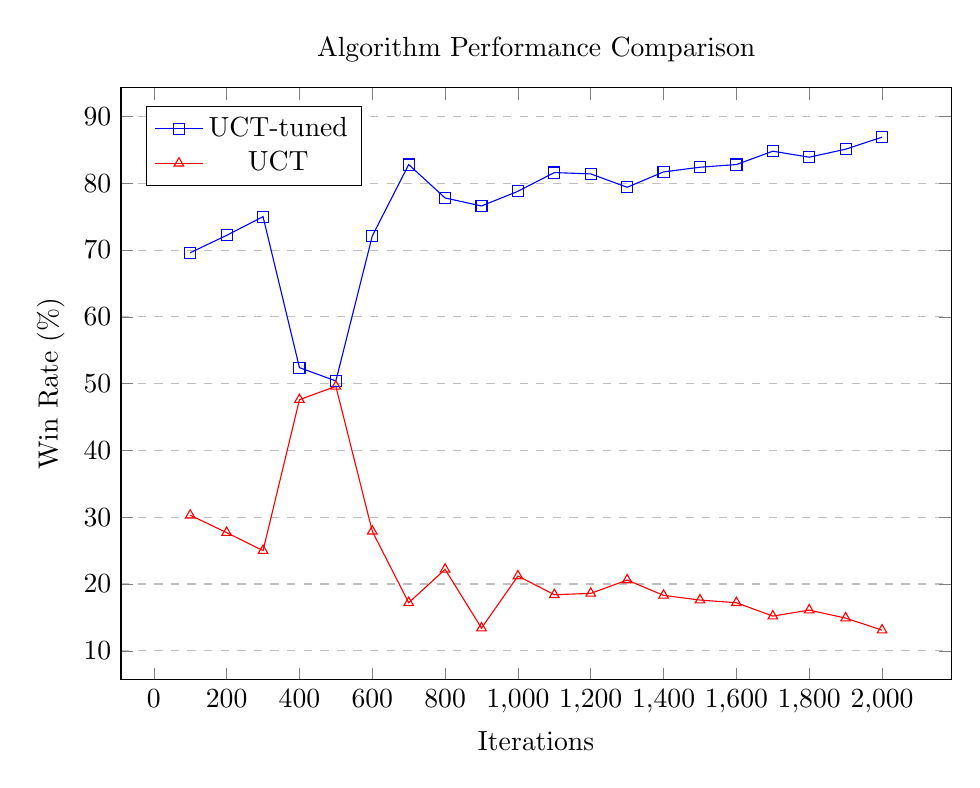
\begin{tikzpicture}
        \begin{axis}[
            title={Algorithm Performance Comparison},
            xlabel={Iterations},
            ylabel={Win Rate (\%)},
            width=\linewidth,
            height=0.75\linewidth,
            legend pos=north west,
            ymajorgrids=true,
            grid style=dashed,
        ]
        \addplot[
            color=blue,
            mark=square,
            ]
            coordinates {
            (100, 69.6)(200, 72.2)(300, 75.0)(400,52.4)(500, 50.4)(600, 72.1)(700, 82.8)(800, 77.8)(900, 76.6)(1000, 78.8)(1100, 81.6)(1200, 81.4)(1300, 79.4)(1400, 81.7)(1500, 82.4)(1600, 82.8)(1700, 84.8)(1800, 83.9)(1900, 85.1)(2000, 86.9)
            };
            \addlegendentry{UCT-tuned}
        \addplot[
            color=red,
            mark=triangle,
            ]
            coordinates {
            (100, 30.3)(200, 27.7)(300, 25.0)(400, 47.6)(500, 49.6)(600, 27.9)(700, 17.2)(800, 22.2)(900, 13.4)(1000,21.2)(1100,18.4)(1200, 18.6)(1300,20.6)(1400,18.3)(1500, 17.6)(1600, 17.2)(1700, 15.2)(1800, 16.1)(1900, 14.9)(2000,13.1)
            };
            \addlegendentry{UCT}
        \end{axis}
    \end{tikzpicture}
    \caption{Win Rate Comparison of UCT and UCT-tuned Algorithms}
    \label{fig:algorithm_comparison}
\end{figure}
The figure illustrates that the UCT-tuned algorithm exhibits a performance dip between 400-500 iterations compared to UCT. This fluctuation supports our hypothesis: the $\min$ term aids in early exploration, while the variance term enhances performance with sufficient iterations, ultimately leading to a higher win rate for UCT-tuned.\\
Additionally, the results demonstrate that UCT-tuned consistently outperforms UCT in terms of win rate as the number of iterations increases. This indicates that the modifications introduced in UCT-tuned, such as the variance tail and adjusted exploration-exploitation balance, provide significant advantages in more complex game scenarios like Gobang. The higher win rates achieved by UCT-tuned in later iterations suggest that it is more effective at identifying and exploiting optimal strategies over time.\\
Overall, the experimental results validate the effectiveness of the UCT-tuned algorithm, highlighting its potential as a superior alternative to traditional UCT in various applications. The integration of advanced techniques and careful parameter tuning in UCT-tuned contribute to its enhanced performance, making it a valuable tool for decision-making in complex environments.
\section{Conclusion}
In this survey, we have explored the intricacies of Monte Carlo Tree Search (MCTS), examining its foundational concepts, algorithmic implementations, and practical applications. We began by discussing the background of MCTS, including the essential elements of Markov Decision Processes (MDP) and Monte Carlo methods, providing a solid foundation for understanding MCTS's operation and relevance in decision-making processes.\\
We introduced the general MCTS algorithm, detailing its four main steps: selection, expansion, simulation, and backpropagation. This was followed by an examination of specific MCTS variants, such as reward-based, visited-based, and hybrid MCTS, highlighting their unique approaches to balancing exploration and exploitation.\\
The survey also covered state-of-the-art algorithms like UCT (Upper Confidence bounds for Trees) and its variations, including UCB1-tuned and Bayesian UCT, analyzing their theoretical foundations, practical implementations, and performance improvements over basic MCTS.\\
Furthermore, we explored the integration of learning techniques within MCTS, such as Temporal Difference (TD) learning and its Monte Carlo variant (TDMC), which enhance the MCTS framework by incorporating value function approximations and reducing variance in value estimation.\\
Our experimental results, particularly in the context of the Tic-Tac-Toe game, demonstrated the effectiveness of advanced MCTS algorithms like UCT and UCB1-tuned, which consistently outperformed simpler variants, showcasing their robustness and adaptability in various scenarios.\\
In conclusion, MCTS remains a powerful and versatile tool in artificial intelligence and decision-making. Its ability to balance exploration and exploitation, coupled with advancements in algorithmic strategies, ensures its continued relevance and applicability in solving complex problems. Future research will likely yield even more sophisticated and efficient algorithms, further expanding the horizons of MCTS.
\bibliography{reference}
\bibliographystyle{plain}
\end{document}
